\chapter{Présentation de l'entreprise d’accueil} % Crée un nouveau chapitre avec ce titre
\begin{spacing}{1.2} % Définit un interligne de 1,2 pour le contenu placé dans cet environnement
	\renewcommand{\mtctitle}{Contenu} % Remplace le titre par défaut de la mini-table des matières par « Contenu »
	\minitoc % Affiche la mini-table des matières du chapitre
	\thispagestyle{MyStyle} % Applique le style de page personnalisé nommé « MyStyle » à cette page
\end{spacing} % Termine l’environnement avec l’interligne de 1,2
\newpage % Commence le contenu suivant sur une nouvelle page


\section{Introduction}
Crée une section principale intitulée "Titre niv 1".

\section{Présentation de ....}
Crée une section principale intitulée "Titre niv 2".

\subsection{Titre niv 2}
Crée une sous-section dans la section précédente, intitulée "Titre niv 2".

\subsubsection{Titre niv 3}
Crée une sous-sous-section dans la sous-section précédente, intitulée "Titre niv 3".
% liste numérotée
\begin{enumerate}
	\item Première étape
	\item Deuxième étape
	\item Troisième étape
\end{enumerate}

% Liste à puces

\begin{itemize}
	\item Première idée
	\item Deuxième idée
\end{itemize}

\section{Images}
Ce bloc de code insère une image dans le document. La figure \ref{f1} présente un diagramme de Gantt utilisé pour la gestion de projet. Ce type de diagramme permet de visualiser les différentes tâches, leurs durées et leurs chevauchements dans le temps \cite{ganttproject}.

Ce diagramme facilite également le suivi de l'avancement du projet en mettant en évidence les différentes phases, les dépendances entre les tâches ainsi que leur durée d'exécution. Il constitue un outil d'aide à la planification et à l'organisation, permettant d'identifier les étapes critiques et de respecter les délais fixés pour la réalisation du projet.

En outre, cette illustration permet au lecteur de mieux comprendre l'organisation temporelle des activités du projet. L'utilisation d'une figure améliore la lisibilité du document en synthétisant des informations qui seraient plus difficiles à interpréter sous forme de texte. Les illustrations constituent ainsi un support visuel essentiel pour faciliter la compréhension des concepts présentés.
\begin{figure}[H] % Commence l’environnement de la figure et impose son emplacement ici
	\centering % Centre l’image horizontalement sur la page
	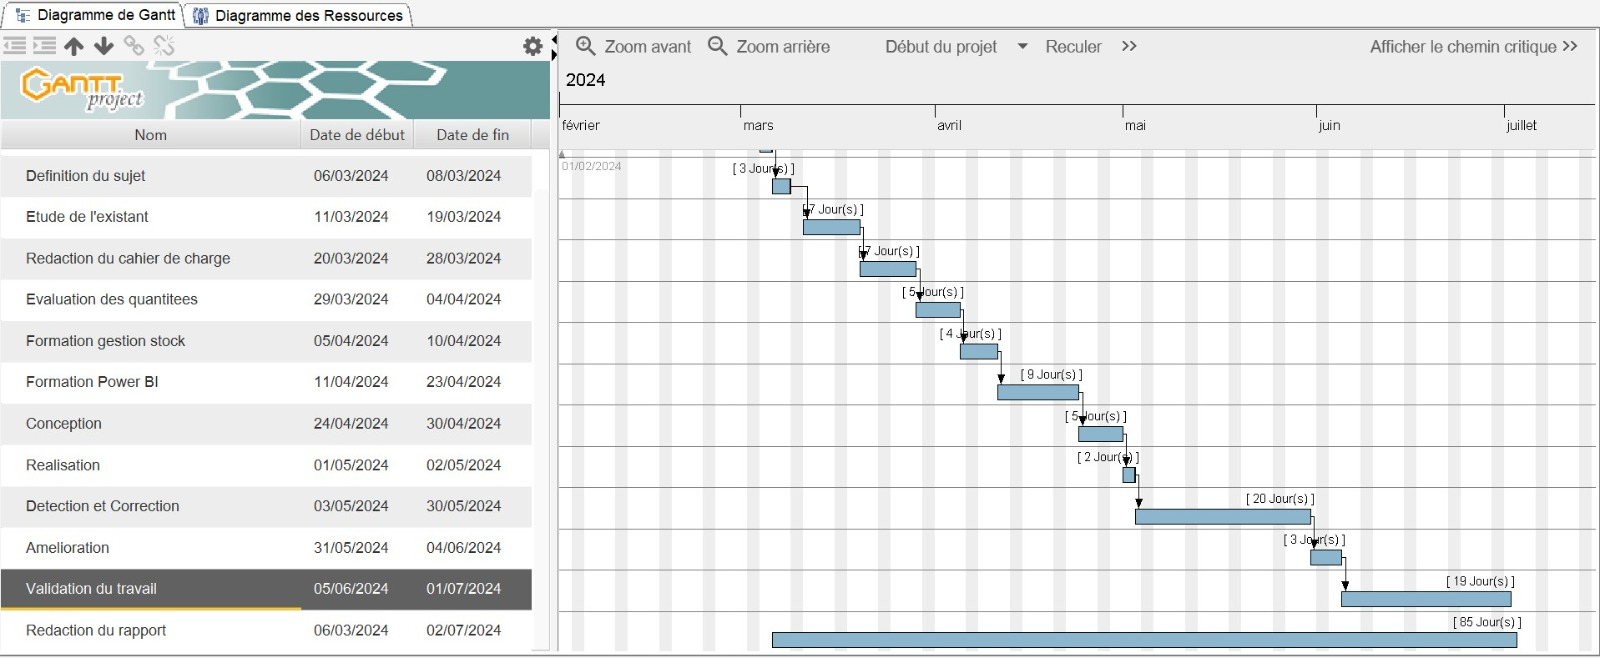
\includegraphics[width=1\textwidth]{images/f1} % Insère l’image avec une largeur égale à 80 % de la largeur du texte
	\caption{Diagramme de Gantt} % Ajoute la légende et le numéro automatique de la figure
	\label{f1} % Donne un identifiant à la figure pour pouvoir la citer dans le texte
\end{figure} % Termine l’environnement de la figure


\begin{figure}[H] % Commence l’environnement de la figure et impose son emplacement ici
	\centering % Centre l’image horizontalement sur la page
	
\includegraphics[width=1\textwidth]{images/ocp} % Insère l’image avec une largeur égale à 80 % de la largeur du texte
	\caption{Image de l'ocp} % Ajoute la légende et le numéro automatique de la figure
	\label{ocp} % Donne un identifiant à la figure pour pouvoir la citer dans le texte
\end{figure} %


\begin{figure}[H] % Commence l’environnement de la figure et impose son emplacement ici
	\centering % Centre l’image horizontalement sur la page
	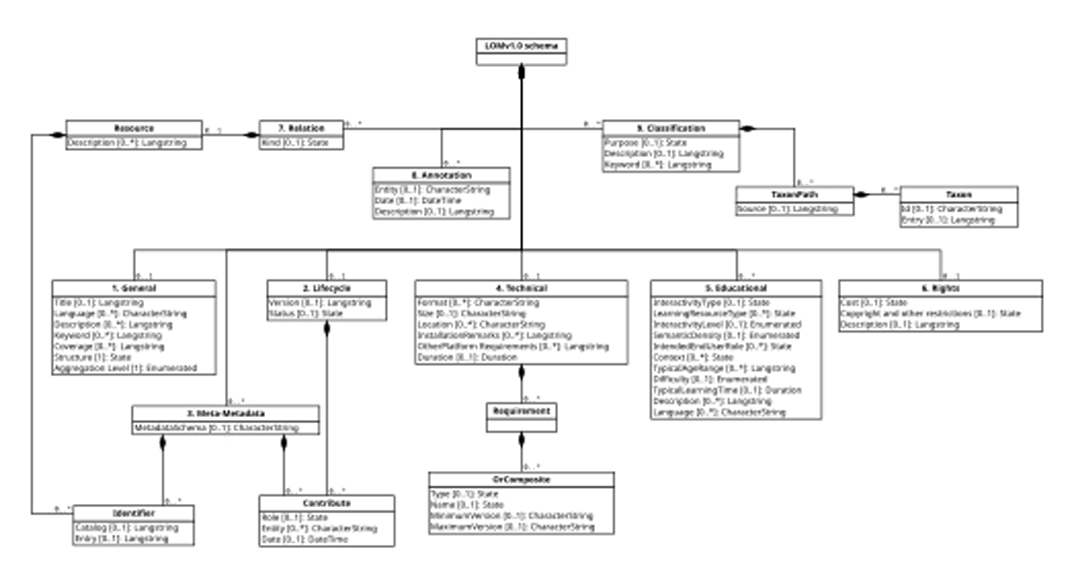
\includegraphics[width=1\textwidth]{images/diag} % Insère l’image avec une largeur égale à 80 % de la largeur du texte
	\caption{Diagramme de classe} % Ajoute la légende et le numéro automatique de la figure
	\label{diag} % Donne un identifiant à la figure pour pouvoir la citer dans le texte
\end{figure} %

La figure \ref{diag} présente le diagramme de classe.\\




La figure \ref{ocp} présente l'image de l'ocp \cite{ocp}.\\
Comme le montre la figure \ref{f1}, un diagramme de Gantt permet de suivre l'avancement des projets, les tâches qui se chevauchent et les dépendances entre elles.

\section{Tableau}
Ce bloc de code insère un tableau sous forme d'image. Le tableau \ref{l1} présente la fiche signalétique du groupe OCP. Ce tableau fournit des informations essentielles sur l'organisation, y compris sa structure et ses principales activités.

\begin{table}[H]
	\centering
	\captionof{table}{Fiche signalétique du groupe OCP}
	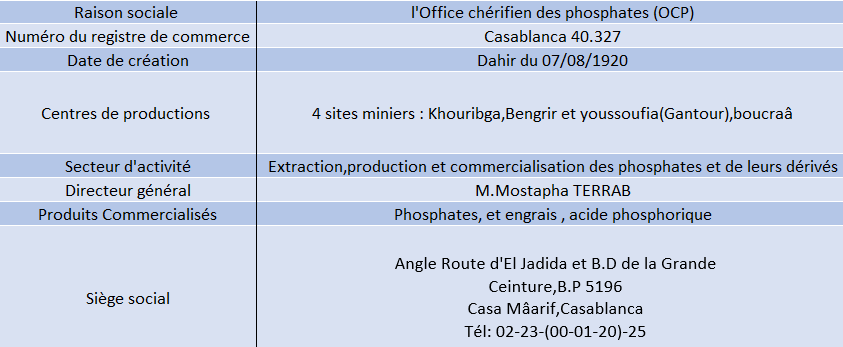
\includegraphics[width=1\textwidth]{images/t1} % Remplacez par le chemin de votre image de tableau
	\label{l1} % Ajout du label pour la référence croisée
\end{table}

\begin{table}[H]
	\centering
	\captionof{table}{Tableau test}
	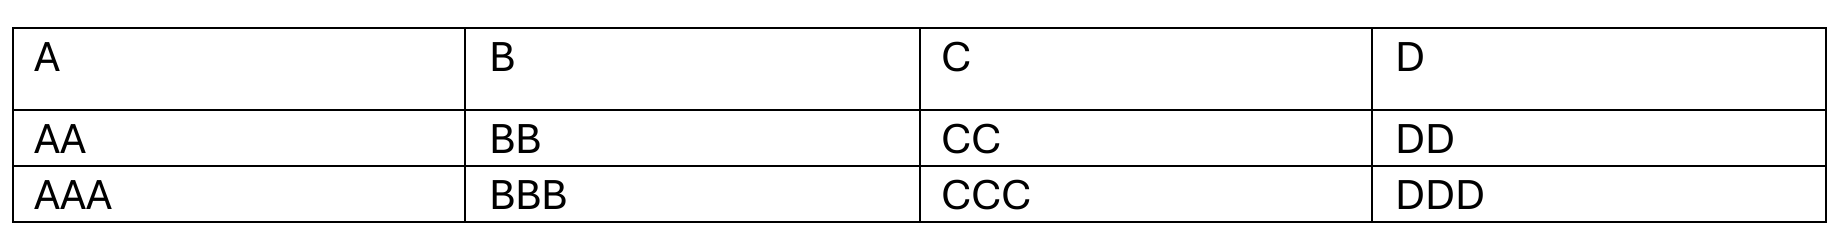
\includegraphics[width=1\textwidth]{images/t2} % Remplacez par le chemin de votre image de tableau
	\label{t2} % Ajout du label pour la référence croisée
\end{table}


\begin{table}[H]
	\centering
	\renewcommand{\arraystretch}{1.2}
	\begin{tabular}{|p{3cm}|p{3cm}|p{3cm}|p{3cm}|}
		\hline
		A   & B   & C   & D   \\ \hline
		AA  & BB  & CC  & DD  \\ \hline
		AAA & BBB & CCC & DDD \\ \hline
	\end{tabular}
\end{table}

Le tableau \ref{t2} présente ... \\
Comme montré dans le tableau \ref{l1}, la fiche signalétique présente les informations clés sur le groupe OCP, telles que sa date de création, son secteur d'activité, et d'autres données importantes.



\section{Conclusion}
xx xxxxx xxxx xxxxx xxxxx xxxxx xxxxxxxxx xxxxx xxxxxxx xxxx xxxxxxxxx xxxxxxx xxxxxx xxxx xxxxxxxxx xxxxxxxx xxxxxxxx xxxxxxxxx xxxxx xxxxxxxxxxx xxxxx xxxxxxx

